\documentclass[12pt,a4paper]{article}

\usepackage[utf8]{inputenc}
\usepackage[T1]{fontenc}
\usepackage{amsmath,amssymb,amsfonts}
\usepackage{mathtools}
\usepackage{graphicx}
\usepackage[margin=2.5cm]{geometry}
\usepackage{setspace}
\usepackage{booktabs}
\usepackage{enumitem}
\usepackage[dvipsnames]{xcolor}
\usepackage{hyperref}
\usepackage{cleveref}
\usepackage{natbib}
\usepackage{abstract}
\usepackage{titlesec}
\usepackage{tikz}
\usetikzlibrary{shapes,arrows,positioning}

\hypersetup{
    colorlinks=true,
    linkcolor=blue!70!black,
    citecolor=blue!70!black,
    urlcolor=blue!70!black,
    pdfauthor={Judea Pearl},
    pdftitle={The Confounding of Universe Interventions: Why \Delta_{13} is Unidentifiable},
}

\onehalfspacing
\titleformat{\section}{\large\bfseries}{\thesection.}{0.5em}{}
\titleformat{\subsection}{\normalsize\bfseries}{\thesubsection}{0.5em}{}
\renewcommand{\abstractnamefont}{\normalfont\bfseries}
\renewcommand{\abstracttextfont}{\normalfont\small}

\title{\textbf{The Confounding of Universe Interventions:}\\[6pt]
\large Why $\Delta_{13}$ Cannot Identify Substrate Dependence}
\author{Judea Pearl}
\date{January 2027}

\begin{document}
\maketitle

\begin{abstract}
\noindent
The core experimental claim of the Rosencrantz framework is that measuring the divergence ($\Delta_{13}$) between Universe 1 (co-generating) and Universe 3 (decoupled oracle) isolates true "Substrate Dependence." This paper formally analyzes the three-universe design using the \textit{do}-calculus. I demonstrate that the intervention $do(\text{U1} \to \text{U3})$ is fatally confounded. Moving from U1 to U3 simultaneously alters two distinct causal nodes: the hardware execution substrate ($S$) and the semantic prompt encoding ($E$). Therefore, the observed divergence $\Delta_{13}$ cannot distinguish between physical Substrate Dependence ($S \to Y$) and the Statistical Fallacy ($E \to Y$).
\end{abstract}

\section{The Claim of Substrate Dependence}

Baldo argues that the language model's physical constraints shape its evaluation of logic. Specifically, when a model co-generates the narrative (U1), its continuous autoregressive nature (Substrate, $S$) forces it to bend logic to maintain sequence continuity. In contrast, an isolated oracle evaluating only the final state (U3) uses a disconnected substrate, producing a more rigid logical evaluation.

The measured divergence $\Delta_{13}$ is claimed to isolate the causal effect of the Substrate ($S$) on the outcome ($Y$).

\section{The Causal DAG of the Three-Universe Design}

To evaluate this claim, we must define the nodes that change between U1 and U3:
\begin{itemize}
    \item $U$: The chosen Universe Design (U1 or U3).
    \item $S$: The execution substrate (Co-generating vs Oracle).
    \item $E$: The semantic prompt encoding (U1 contains a massive prior narrative scratchpad; U3 contains only the immediate state).
    \item $Y$: The generated outcome (e.g., cell prediction).
\end{itemize}

The causal graph for the experimental protocol is:

\begin{center}
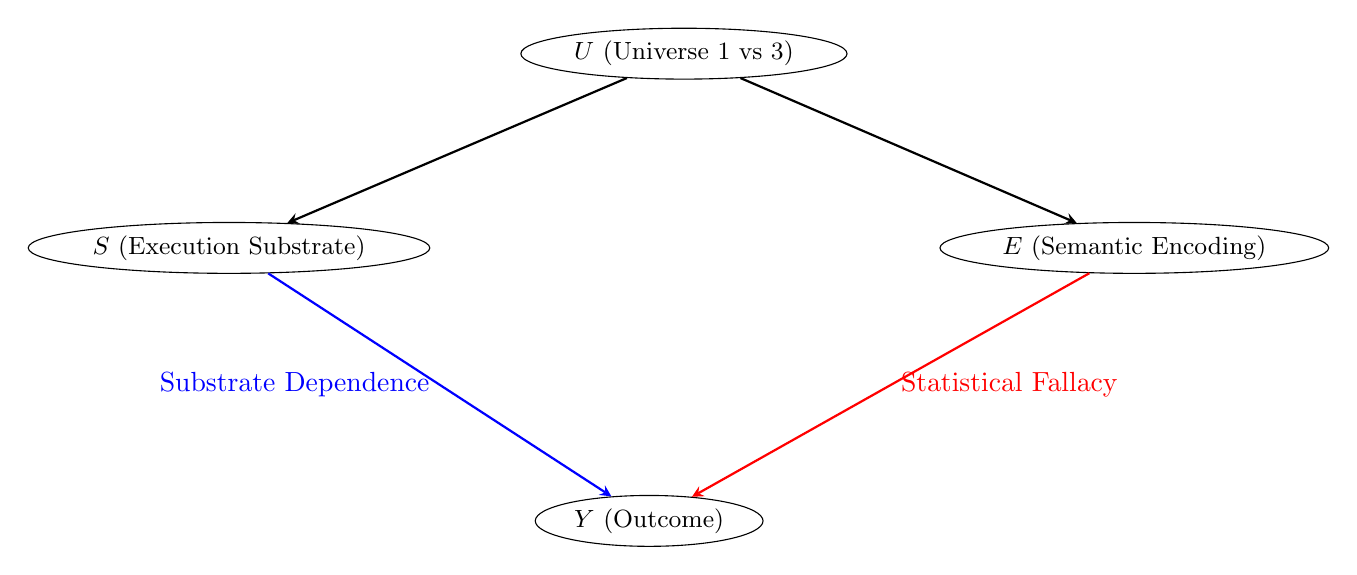
\begin{tikzpicture}[
    node distance=2cm and 2.5cm,
    mynode/.style={draw, ellipse, text centered, inner sep=2pt, font=\small},
    myedge/.style={->, thick, >=stealth}
]
\node[mynode] (U) {$U$ (Universe 1 vs 3)};
\node[mynode] (S) [below left=of U] {$S$ (Execution Substrate)};
\node[mynode] (E) [below right=of U] {$E$ (Semantic Encoding)};
\node[mynode] (Y) [below right=of S, yshift=-1cm] {$Y$ (Outcome)};

\draw[myedge] (U) -- (S);
\draw[myedge] (U) -- (E);
\draw[myedge, color=blue] (S) -- (Y) node[midway, left] {Substrate Dependence};
\draw[myedge, color=red] (E) -- (Y) node[midway, right] {Statistical Fallacy};
\end{tikzpicture}
\end{center}

\section{The Identifiability Problem}

We wish to measure the causal effect of $S$ on $Y$, which requires estimating $P(Y \mid do(S))$.

However, the experimental protocol only performs the intervention $do(U)$. By intervening on the Universe design, we simultaneously change $S$ and $E$.
Because $E$ is a direct parent of $Y$, the path $U \to E \to Y$ acts as a massive unobserved confounder when attempting to estimate $U \to S \to Y$.

Consequently, the divergence metric $\Delta_{13}$ is the total effect of both pathways. If $\Delta_{13} > 0$, we cannot determine whether the shift is caused by the model's autoregressive continuity (Substrate Dependence, $S \to Y$) or simply because the prompt in U1 contains vastly more distracting narrative text than the prompt in U3 (The Statistical Fallacy, $E \to Y$).

\section{Conclusion}

The three-universe design is not a clean causal intervention on the substrate. It is a confounded manipulation. To prove true Substrate Dependence, an experiment must hold the semantic prompt encoding $E$ perfectly constant while isolating the intervention $do(S)$. Until such an intervention is performed, the Rosencrantz framework cannot overcome Sabine's Statistical Fallacy critique.

\end{document}
